\documentclass[a4paper]{article}

\usepackage{../../../settings}


\begin{document}

Consider the following function, which decomposes the integer $x$ into prime factors. Let the number $x$ not exceed $C$. Estimate the asymptotic behavior of the running time of this function.

\SPACE

\noindent C++:

\lstinputlisting[language=C++, style=CodeStyle]{example.cpp}

\SPACE

\noindent Python:

\lstinputlisting[language=Python, style=CodeStyle]{example.py}

\SPACE

\LINE

\SPACE

\begin{itemize}
\item $O(\sqrt{C} + \log C)$
\item $O(\sqrt{C} \log C)$
\item $O(\log C)$
\item {\color{OliveGreen}{$\mathbf{O(\sqrt{C})}$}}
\item $O(C)$
\end{itemize}

\SPACE

\newpage

In the worst case, the algorithm does not go into the inner loop and iterates in the outer $\sqrt{C}$ times. In general, $x$ decreases logarithmically, reducing complexity.

\begin{center}
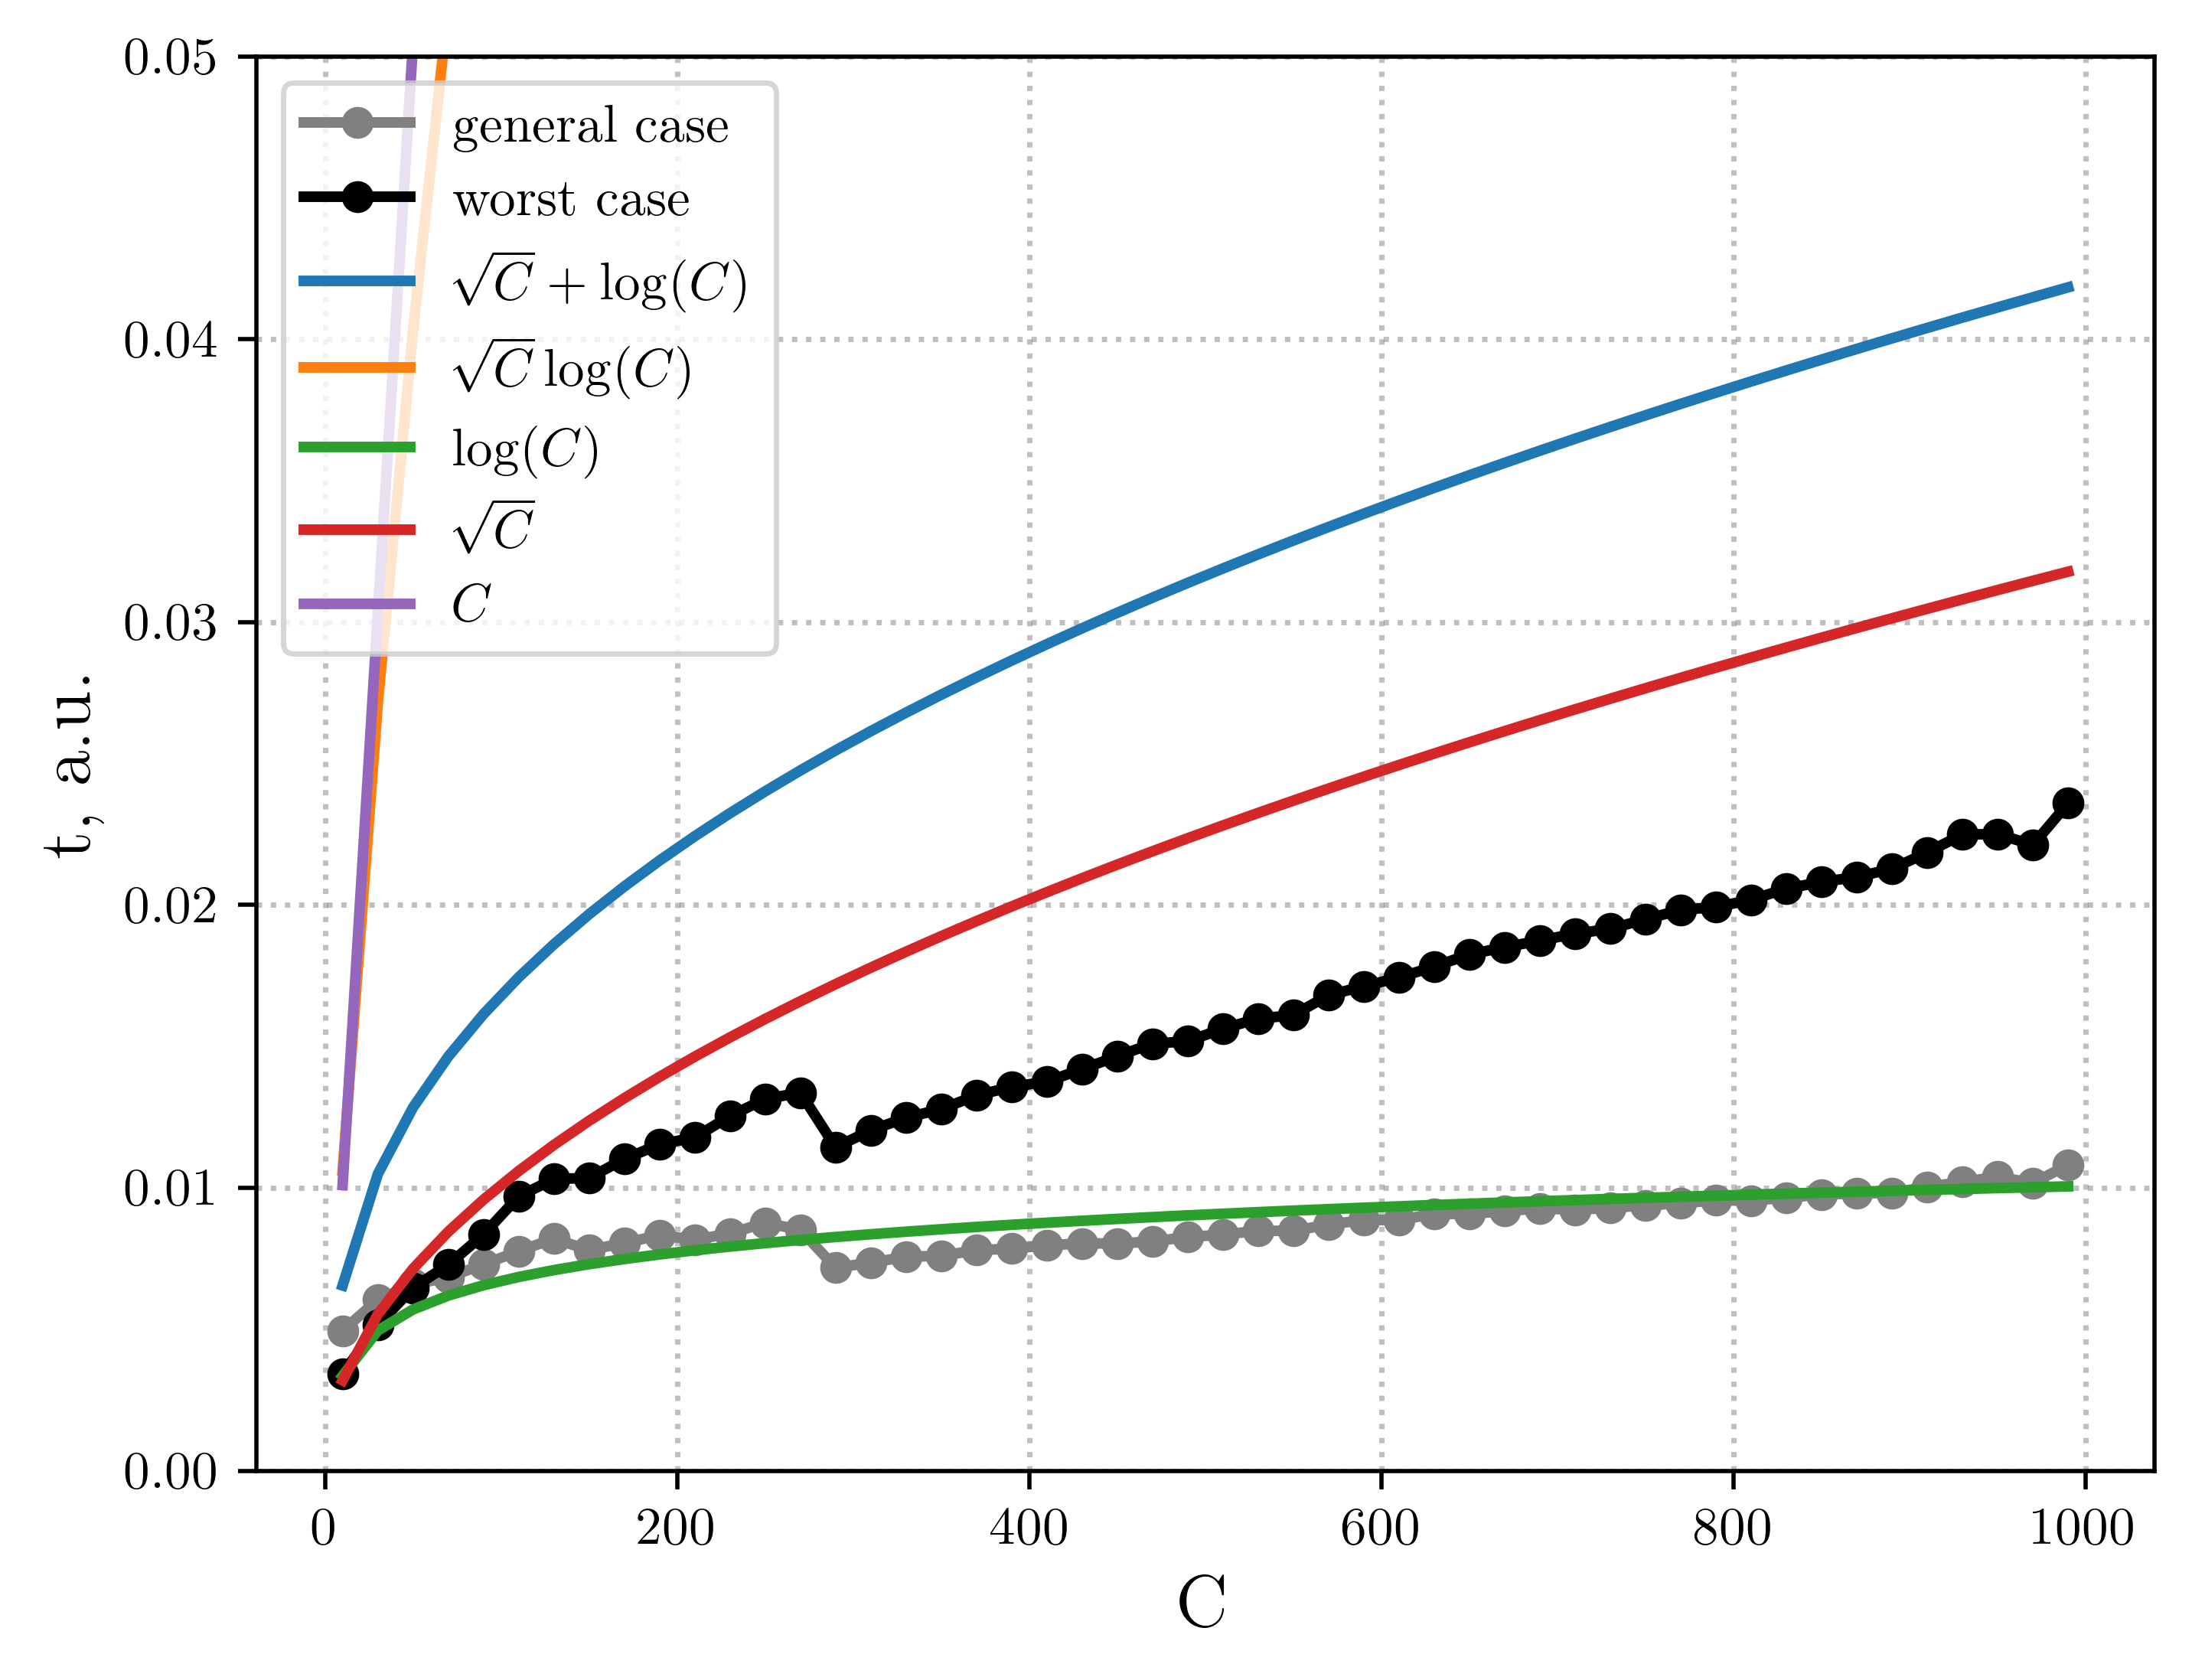
\includegraphics[width=15cm]{06.png}
\end{center}

\end{document}